%%==================================================
%% chapter04.tex for SJTU Master Thesis
%% based on CASthesis
%% modified by wei.jianwen@gmail.com
%% version: 0.3a
%% Encoding: UTF-8
%% last update: Dec 5th, 2010
%%==================================================

% \bibliographystyle{sjtu2} %[此处用于每章都生产参考文献]
\raggedbottom
\chapter{DiffCon的设计与实现}
\label{chap:designandimpl}

\section{引言}

前文总结了课题相关的基础算法和优化思路之间的联系和启发,探讨了范围查询需求和算法的数据组织形式之间的关联点,本章节以优化频率矩阵加噪模型、提升发布数据可用性为目的,论述解决方案——非交互式差分隐私匿名优化算法DiffCon的设计和实现。

本章节将从基础算法出发,从基于一致性约束的噪音调整、重定义加噪方式以及优化算法的组合应答模式这几个方面介绍DiffCon算法,并就其关键技术、难点等作分析。

\section{基础算法概览}

面向分类应用的非交互式差分隐私匿名算法DiffGen主要的流程为:(1)为每个属性定义匿名树结构,得到匿名树森林,并定义树高。(2)基于决策树算法构建分类树并逐层划分数据集。(3)由叶节点的类属性计数生成发布数据集。流程伪代码\ref{totalprocedure}概括如下:

\begin{algorithm}
	\caption{DiffGen算法流程} 
	\label{totalprocedure}
	\begin{algorithmic}[1]
		\REQUIRE 隐私代价$\varepsilon$,树高$Hight$,数据集,匿名树森林。
		\ENSURE 发布数据集。
		\STATE 定义合理数据结构处理数据集和匿名树森林,并建立相应联系
		\STATE 初始化分类树根节点,记当前树高为$h$
		\WHILE{$h++$ < $Hight$} 
		\STATE 基于决策树算法,逐层选择属性、分裂当前节点并划分父节点数据集,构建分类树。
		\ENDWHILE
		\STATE 在分类树叶子节点的类属性计数上添加拉普拉斯噪音,全局敏感性为1。
		\STATE 遍历叶节点,根据类属性计数值生成匿名化数据集
		\RETURN 发布数据集
	\end{algorithmic}
\end{algorithm}

\subsection{匿名树的维护}

匿名规则需要数据发布者自己定义,算法读取语义文件并构建匿名树。属性分为连续属性(Numerical attribute)和离散属性(Categorical attribute)两类,如年龄、身高属于连续属性,国籍、肤色属于离散属性。选取真实数据集adult\cite{adult}中的离散属性relationship和连续属性age作为示例,如图\ref{fig4:attribute}。图\ref{fig4:semantic}是对应的自定义匿名结构语义,通过“\{”和“\}"分层。

\begin{figure}[!htp]
	\centering
	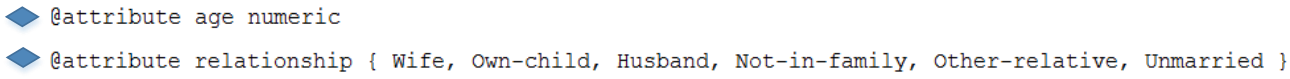
\includegraphics[width=5.5in]{chap4/attribute}
	\bicaption[fig4:attribute]{图}{连续和离散属性及其属性值}{Fig.}{numerical/categorical attribute and attribute value}
\end{figure}


\begin{figure}[!htp]
	\centering
	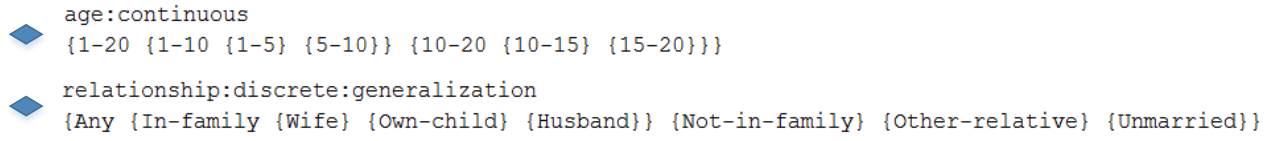
\includegraphics[width=5.5in]{chap4/semantic}
	\bicaption[fig4:semantic]{图}{属性的自定义匿名化结构语义}{Fig.}{The user-defined semantics of anonymous structure for attribute}
\end{figure}

DiffGen读取并解析匿名结构语义后,构建如图\ref{fig4:relationship}、图\ref{fig4:age}的匿名树,作为属性切割、数据集划分的依据。匿名树的叶节点用气泡框标识,也是最“细”的发布属性值。

\begin{figure}[!htp]
	\centering
	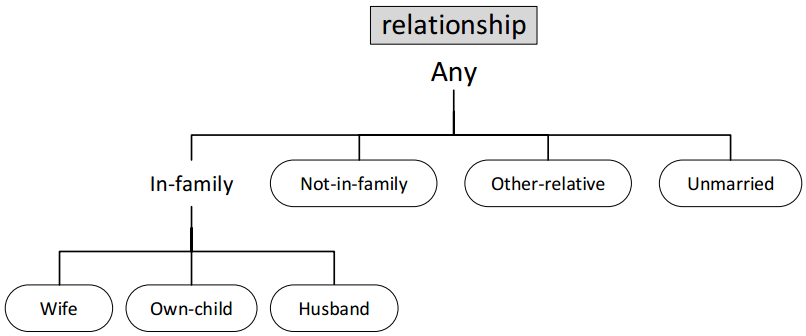
\includegraphics[width=5in]{chap4/relationship}
	\bicaption[fig4:relationship]{图}{根据属性relationship的匿名语义构建的匿名树}{Fig.}{A taxonomy tree for attribute relationship that is built by anonymous semantics}
\end{figure}

\begin{figure}[!htp]
	\centering
	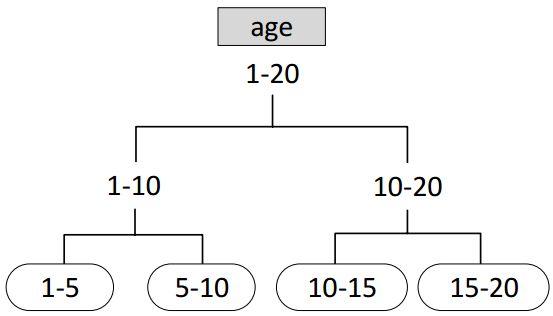
\includegraphics[width=3.5in]{chap4/age}
	\bicaption[fig4:age]{图}{根据属性age的匿名语义构建的匿名树}{Fig.}{A taxonomy tree for attribute age that is built by anonymous semantics}
\end{figure}

\subsection{算法框架与一致性特性}

在这个阶段,DiffGen算法依据匿名树的分裂规则,采用决策树算法通过指数机制逐层选择分裂属性,并作数据集划分,构建完整的分类树,最后在叶节点加噪并发布数据集。为了更清楚地展示这个过程以及理解DiffGen算法伪代码,继续使用前文公司应聘的例子做说明。
\begin{exmp}
	\label{chap4_exmp}
	某公司有8位应聘者,对属性“国籍”、“年龄”以及是否被成功录用做统计,类属性值的“是”、“否”表示为是否被录用。
\end{exmp}

图\ref{fig4:diffgen}展示了示例\ref{chap4_exmp}背景下的算法工作过程。算法\ref{diffgen}对DiffGen算法进行了完整描述,其中$Cut_{i}$表示在当分类树树高为i时,所有匿名树中可分裂的属性集合。如,仅有根节点时,$Cut_{1}$=\{亚洲,[15-40)\};而选取分裂属性亚洲后,$Cut_{2}$=\{东亚,西亚,[15-40)\}。$u(D,\cdotp)$表示打分函数,$S(u)$为其全局敏感性。


\begin{algorithm}
	\caption{DiffGen算法} 
	\label{diffgen}
	\begin{algorithmic}[1]
		\REQUIRE 隐私代价$\varepsilon$,树高$Hight$,数据集$D$。
		\ENSURE 新的匿名数据集$\hat{D}$。
		\STATE 初始化分类树根节点和$Cut_{i}$集合,此时i=1
		\STATE 按树高切割$\varepsilon\textasciiacute$,统计连续属性个数为$A_{Pr}^{n}$,$\varepsilon$' $\leftarrow$ $\frac{\varepsilon}{2(|A_{Pr}^{n}|+2Hight)}$
		\STATE 对$Cut_{i}$里的每个连续属性$v_{n}$,计算其分裂点$p$,分裂点$p$的选中概率 $\wasypropto$ exp($\frac{\varepsilon\textasciiacute}{2S(u)}$$u(D,v_{n})$)
		\STATE 对所有的属性$v$, $\forall$$v$ $\in$ $Cut_{i}$,计算分值
		\FOR{i = 1 to $Hight$}
		\STATE 按分值选择属性$v$,$v$$\in$ $Cut_{i}$,且$v$的选中概率$\wasypropto$ exp($\frac{\varepsilon\textasciiacute}{2S(u)}$$u(D,v)$)
		\STATE 根据$v$的匿名树分裂节点$v$,$v$$\rightarrow$$child(v)$
		\STATE $Cut_{i}$ $\leftarrow$ $Cut_{i}$$ - $$v$,$Cut_{i}$ $\leftarrow$ $Cut_{i}$ $\cup$ $child(v)$
		\STATE 对$Cut_{i}$里的新出现的连续属性$v_{n}$,计算其分裂点$p$,分裂点$p$的选中概率 $\wasypropto$ exp($\frac{\varepsilon\textasciiacute}{2S(u)}$$u(D,v_{n})$)
		\STATE 对所有的属性$v$, $\forall$$v$ $\in$ $Cut_{i}$,更新分值
		\ENDFOR
		\RETURN 在叶子节点的数据项上,每个类属性计数为$C$,返回($C$+Laplace(1/$\varepsilon$))
	\end{algorithmic}
\end{algorithm}

在算法\ref{diffgen}中,选取分裂属性和处理连续属性分裂点时需要消耗隐私预算,因此在第2行对隐私预算进行了切分。在5-10行的每次迭代中,需要先对待选择属性集$Cut_{i}$的每个属性计算分值并对连续属性处理进行处理,然后通过指数机制按概率挑选属性。在第8行进行更新$Cut_{i}$集合操作,第9,10行更新分值。第12行在每个叶节点类属性计数上添加独立的拉普拉斯噪音,并返回。最后,在数据集发布阶段,根据类计数分布逐条发布匿名化数据集,如图\ref{fig4:diffgen}的下半部分所示。

\begin{figure}[!htp]
	\centering
	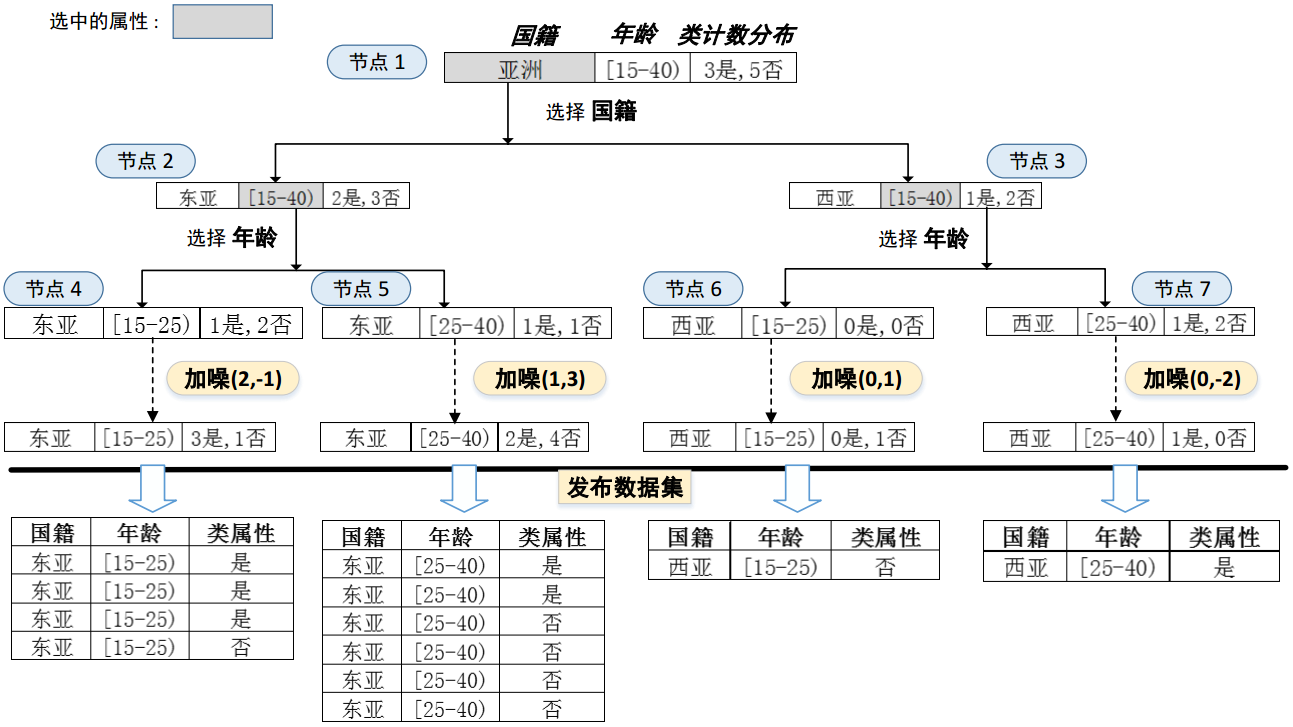
\includegraphics[width=6.2in]{chap4/diffgen}
	\bicaption[fig4:diffgen]{图}{DiffGen算法流程示例}{Fig.}{A sample for the procedure of DiffGen}
\end{figure}

泛化技术和决策树分类方式决定了DiffGen算法的数据项之间具有一致性关系,在图\ref{fig4:diffgen}中可以清楚地看到父子节点间的这种约束关系。例如,对于[东亚,[15-40)]的范围查询请求,节点2可直接满足查询需求,它等价于节点4和节点5的累加运算,因为基于“年龄”属性的匿名树在节点2上对“$[15-40)$”进行分裂,且生成的节点4,5是唯一的。


\section{基于一致性约束的优化算法DiffCon}

针对范围计数查询应用,从基础算法出发,本节就基于一致性约束的优化思路,对非交互式差分隐私优化算法DiffCon的总体设计思进行详细阐述。主要分为以下几个部分:
\begin{enumerate}
	\item 立足于DiffGen的分类树结构,它是对原始数据集进行重匿名划分、生成新数据集的重要途径,是实施新的加噪方式的底层结构,是对外应答处理的算法基础。
	\item 改变基于数据条目的独立加噪方式,对分类树的每个节点均进行加噪处理,重定义全局敏感性。
	\item 设计并实现基于任意树结构的噪音调整算法,通过一致性约束优化噪音分布,使之更加合理。
	\item 基于分类树结构,对于范围查询可利用内部节点进行间接应答。展示DiffCon的组合应答模式及其处理算法。
\end{enumerate}

\subsection{分类树基础}

DiffGen分类树是本课题优化算法的基础结构,噪音分布、优化技术以及查询应答原理均基于此。因此,以DiffGen的匿名树设计和分类树构建算法\ref{diffgen}为基础,DiffCon在生成分类树的同时维护树形结构$DTree$。它可以看成是加噪、发布处理前分类树,但是额外维护了$LapNoise$和$OptNoise$两个变量,分别表示


\subsection{全局敏感性的重定义}

应说清 为了利用一致性进行应答,因此全局敏感要改,但是还是落在叶节点上。

\subsection{噪音调整算法}

\subsection{组合应答模式}

\subsection{流程总结}

\section{本章小结}